\documentclass[12pt]{article} % use larger type; default would be 10pt
\usepackage[czech]{babel}
\usepackage[utf8]{inputenc} % set input encoding (not needed with XeLaTeX)

%%% PAGE DIMENSIONS
\usepackage{geometry} % to change the page dimensions
% \usepackage[left=2cm,right=2cm,top=2cm,bottom=2cm]{geometry}
\geometry{a4paper}
% \geometry{margin=2in} % for example, change the margins to 2 inches all round
% \geometry{landscape} % set up the page for landscape

\usepackage{graphicx} % support the \includegraphics command and options
\usepackage{wrapfig} % support the wrapfigure section

\usepackage{tikz} % graphs
\usepackage{pgfplots}

\usepackage{hyperref} % links in \tableofcontents
\hypersetup{
	colorlinks,
	citecolor=black,
	filecolor=black,
	linkcolor=black,
	urlcolor=black
}

% \usepackage[parfill]{parskip} % Activate to begin paragraphs with an empty line rather than an indent

%%% PACKAGES
\usepackage{booktabs} % for much better looking tables
\usepackage{array} % for better arrays (eg matrices) in maths
% \usepackage{paralist} % very flexible & customisable lists (eg. enumerate/itemize, etc.)
\usepackage{verbatim} % adds environment for commenting out blocks of text & for better verbatim
\usepackage{subfig} % make it possible to include more than one captioned figure/table in a single float
% These packages are all incorporated in the memoir class to one degree or another...
\usepackage{float}

%%% HEADERS & FOOTERS
\usepackage{fancyhdr} % This should be set AFTER setting up the page geometry
\pagestyle{fancy} % options: empty , plain , fancy
\renewcommand{\headrulewidth}{0pt} % customise the layout...
\lhead{}\chead{}\rhead{}
\lfoot{}\cfoot{\thepage}\rfoot{}

%%% SECTION TITLE APPEARANCE
\usepackage{sectsty}
\allsectionsfont{\sffamily\mdseries\upshape} % (See the fntguide.pdf for font help)
% (This matches ConTeXt defaults)

%%% ToC (table of contents) APPEARANCE
\usepackage[nottoc,notlof,notlot]{tocbibind} % Put the bibliography in the ToC
\usepackage[titles,subfigure]{tocloft} % Alter the style of the Table of Contents
\renewcommand{\cftsecfont}{\rmfamily\mdseries\upshape}
\renewcommand{\cftsecpagefont}{\rmfamily\mdseries\upshape} % No bold!
\newcommand{\bigsize}{\fontsize{35pt}{20pt}\selectfont}

%%% END Article customizations

\begin{document}
\begin{titlepage}
	
\includegraphics[scale=0.7]{logo.jpg}
	\vspace*{\fill}
	\begin{center}
		\textsc{\LARGE \bigsize Měření impedance třemi voltmetry}\\[1cm]
		Martin Zlámal \\[1cm]
		{\small\em \copyright \ Datum poslední revize \today } \\
		\LaTeX
	\end{center}
	\vspace*{\fill}
\end{titlepage}
\tableofcontents
\listoffigures
\listoftables
\newpage

\section{Zadání}
\begin{enumerate}
\item Metodou třech voltmetrů změřte impedanci předložené cívky. Určete činný odpor,
reaktanci při kmitočtu $50Hz$ a indukčnost cívky.
\item Měření opakujte pro tři různé odpory pomocného normálu odporu $R_N$.
\item Změřená napětí a dopočítaný proud zakreslete do fázorových diagramů.
\item Stanovte pro jakou hodnotu normálu $R_N$ je měření nejpřesnější.
\end{enumerate}

\section{Teoretický úvod}
\begin{description}
\item[Metody měření impedancí] \hfill \\
Impedanci měříme při střídavém proudu, aby nedošlo pouze ke změření činné složky impedance. Měřiti můžeme například voltmetrem, ampérmetrem a wattmetrem, nebo pomocí tří ampérmetrů, popř. voltmetrů, což je způsob řešení v této práci. Impedance se dají také měřit číslicově případně můstkem.
\item[Metoda tří voltmetrů] \hfill \\
Meřená impedance je zapojena v sérii s odporovým normálem. Pomocí tří voltmetrů měříme efektivní hodnoty úbytků napětí na normálu, měřené impedanci a napětí celkové.
\item[Náhradní zapojení cívky] \hfill \\
Náhradním zapojením cívky myslíme zapojení ideální cívky do série s s odporem vlastního vinutí. V takovém případě je $Z=R+j\omega L$. Velikost impedance je v tomto případě $|Z|=\sqrt{R^2 + \omega^2 L^2}$. Pro případ zapojení ideální cívky paralelně k odporu vlastního vinutí by platilo, že $Z=\frac{j\omega RL}{R+j\omega L}$. V takovém případě je velikost impedance $|Z|=\frac{|\omega RL|}{\sqrt{R^2 + \omega^2 L^2}}$.
\end{description}

\section{Schéma zapojení}
\begin{figure}[H]
\center
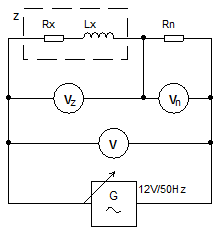
\includegraphics[scale=1]{schema.png}
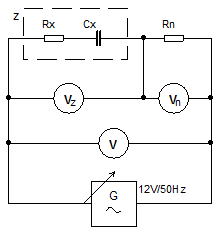
\includegraphics[scale=1]{schema2.png}
\caption{Schéma zapojení}
\end{figure}

\section{Postup měření}
Při měření byl k dispozici pouze jeden voltmetr, takže obvod zapojíme podle schématu, ale vždy budeme měnit pozici voltmetru. Do tabulky si zaznamenáváme jednotlivé hodnoty napětí na normálovém odporu $U_N$, napětí na imepdanci $U_Z$ a celkové  napetí $U$ vždy k příslušné hodnotě normálového odporu. Celé měření provádíme celkem dvakrát. Jednou pro předložený induktor a podruhé pro předložený kapacitor.

\section{Naměřené a dopočítané hodnoty}
\captionof{table}{Naměřené a dopočítané hodnoty pro induktor}
\begin{tabular}{|c|c|c|c|}
\hline 
$R_N [\Omega]$ & 10 & 100 & 1000 \\ 
\hline 
$U [V]$ & 12,740 & 12,799 & 12,160 \\ 
\hline 
$U_N [V]$ & 1,752 & 8,015 & 12,140 \\ 
\hline 
$U_Z [V]$ & 11,080 & 5,053 & 0,770 \\ 
\hline 
$I [A]$ & 0,172 & 0,080 & 0,012 \\ 
\hline 
$Z [\Omega]$ & 64,419 & 63,163 & 64,167 \\ 
\hline 
$\cos \varphi [-]$ & 0,939 & 0,914 & -0,006 \\ 
\hline 
$\varphi [^{\circ}]$ & 20,116 & 23,936 & 90,327 \\ 
\hline 
$R [\Omega]$ & 60,489 & 57,731 & -0,366 \\ 
\hline 
$X [\Omega]$ & 22,155 & 25,626 & 64,166 \\ 
\hline 
$L [H]$ & 0,071 & 0,082 & 0,204 \\ 
\hline 
\end{tabular} \\\\

Velikost proudu impedancí:
\begin{equation}
I = \frac{U_N}{R_N} = \frac{1,752}{10} = 0,175 \Omega
\end{equation}
Velikost impedance:
\begin{equation}
U = \frac{U_Z}{I} = \frac{11,080}{0,172} = 64,419 \Omega
\end{equation}
Účiník:
\begin{equation}
\cos \varphi = \frac{U^2-U_N^2-U_Z^2}{2U_ZU_N} = \frac{12,740^2-1,752^2-11,080^2}{2\cdot 11,080 \cdot 1,752} = 0,939
\end{equation}
Fázový posuv $U_Z$ vůči $I$:
\begin{equation}
\varphi = \arccos(\cos \varphi) = \arccos(0,939) = 20,116^{\circ}
\end{equation}
Činný odpor cívky:
\begin{equation}
R = Z \cos \varphi = 64,419 \cdot 0,939 = 60,489 \Omega
\end{equation}
Reaktance cívky:
\begin{equation}
X = Z \sin \varphi = 64,419 \cdot \sin(20,116) = 22,155 \Omega
\end{equation}
Indukčnost cívky:
\begin{equation}
L = \frac{X}{2\pi f} = \frac{22,155}{2\pi \cdot 50} = 0,071H
\end{equation}

\captionof{table}{Naměřené a dopočítané hodnoty pro kapacitor}
\begin{tabular}{|c|c|c|c|}
\hline 
$R_N [\Omega]$ & 10 & 100 & 1000 \\ 
\hline 
$U [V]$ & 12,885 & 12,862 & 12,880 \\ 
\hline 
$U_N [V]$ & 0,692 & 6,010 & 12,620 \\ 
\hline 
$U_Z [V]$ & 12,868 & 11,278 & 2,368 \\ 
\hline 
$I [A]$ & 0,172 & 0,080 & 0,012 \\ 
\hline 
$Z [\Omega]$ & 64,419 & 63,163 & 64,167 \\ 
\hline 
$\cos \varphi [-]$ & 0,939 & 0,914 & -0,006 \\ 
\hline 
$\varphi [^{\circ}]$ & 20,116 & 23,936 & 90,327 \\ 
\hline 
$R [\Omega]$ & 60,489 & 57,731 & -0,366 \\ 
\hline 
$X [\Omega]$ & 22,155 & 25,626 & 64,166 \\ 
\hline 
$L [H]$ & 0,071 & 0,082 & 0,204 \\ 
\hline 
\end{tabular} \\\\

\section{Grafy}
\begin{figure}[H]
\centering
	\begin{tikzpicture}
		\begin{axis}[
			width=1\textwidth,
	      	height=0.5\textwidth,
			xlabel={$I$},
			ylabel={$L$}]
		\addplot[color=red,mark=x] coordinates {
			(0.009,10.23)
			(0.020,13.71)
			(0.025,14.64)
			(0.032,15.32)
			(0.038,16.15)
			(0.045,16.43)
		};
		\addlegendentry{$L=f(I)$}
		\end{axis}
	\end{tikzpicture}
	\caption{Závislost $L=f(I)$}
\end{figure}

\section{Závěr}

\section{Přístroje}
\begin{itemize}
\item Multimetr Escort 1136A, evid. 177208
\item Zdroj AC/DC 3-24/1,5A, evid. 117254
\item Odporové normály $10,100,1000\Omega - 10W$
\end{itemize}

\end{document}
